\documentclass[10pt,a4paper]{report}
\usepackage{fontspec}
\usepackage{fancyhdr}
\usepackage{booktabs}
\usepackage{geometry}
\usepackage{pdfpages}
\usepackage{csquotes}

\usepackage{xeCJK}  % 使用xeCJK包处理CJK字符
\usepackage{titlesec}  % 使用titlesec包定义标题格式
\usepackage{ctex}
\usepackage{float} % 需要这个包来使用 H 选项
\usepackage{fancyhdr}
\usepackage{titletoc}
\usepackage{xcolor}  % 引入颜色包
\usepackage{setspace}
\usepackage[backend=biber,style=numeric,sorting=none]{biblatex}  % 使用biblatex包管理引用
\addbibresource{references.bib}  % 引用.bib文件
\usepackage{tikz}
\usepackage{pgfplots}
\pgfplotsset{compat=1.17}
\usepackage{caption}
\usepackage{indentfirst}
\setlength{\parindent}{2em}

\setCJKfamilyfont{SimSun}[BoldFont=SimHei]{SimSun}
\setCJKfamilyfont{HeiTi}{SimHei}
\setCJKfamilyfont{KaiTi}{KaiTi}
\setCJKfamilyfont{timesnewroman}{Times New Roman}

\newcommand{\upcite}[1]{\textsuperscript{\cite{#1}}}

% 创建方便使用的命令
\newcommand{\SimSun}{\CJKfamily{SimSun}}
\newcommand{\SimHei}{\CJKfamily{HeiTi}}
\newcommand{\KaiTi}{\CJKfamily{KaiTi}}
\newcommand{\timesnewroman}{\CJKfamily{timesnewroman}}

\DeclareMathSizes{12}{12}{10}{8}

\captionsetup[figure]{labelformat=empty} % 去掉默认图号

\usetikzlibrary{arrows.meta, positioning, fit, shapes.multipart}

\usepackage{adjustbox}
\usetikzlibrary{shapes.geometric, arrows}

\tikzstyle{startstop} = [rectangle, rounded corners, minimum width=3cm, minimum height=1cm,text centered, draw=black, fill=red!30]
\tikzstyle{process} = [rectangle, minimum width=3cm, minimum height=1cm, text centered, draw=black, fill=orange!30]
\tikzstyle{io} = [trapezium, trapezium left angle=70, trapezium right angle=110, minimum width=3cm, minimum height=1cm, text centered, draw=black, fill=blue!30]
\tikzstyle{decision} = [diamond, minimum width=3cm, minimum height=1cm, text centered, draw=black, fill=green!30]
\tikzstyle{arrow} = [thick,->,>=stealth]

% Options for packages loaded elsewhere
\PassOptionsToPackage{unicode}{hyperref}
\PassOptionsToPackage{hyphens}{url}
%
\usepackage{unicode-math}
\usepackage{amsmath}
\usepackage{iftex}
\ifPDFTeX
  \usepackage[T1]{fontenc}
  \usepackage[utf8]{inputenc}
  \usepackage{textcomp} % provide euro and other symbols
\else % if luatex or xetex
  \usepackage{unicode-math} % this also loads fontspec
  \defaultfontfeatures{Scale=MatchLowercase}
  \defaultfontfeatures[\rmfamily]{Ligatures=TeX,Scale=1}
\fi
\usepackage{lmodern}
\ifPDFTeX\else
  % xetex/luatex font selection
\fi
% Use upquote if available, for straight quotes in verbatim environments
\IfFileExists{upquote.sty}{\usepackage{upquote}}{}
\IfFileExists{microtype.sty}{% use microtype if available
  \usepackage[]{microtype}
  \UseMicrotypeSet[protrusion]{basicmath} % disable protrusion for tt fonts
}{}
\makeatletter
\@ifundefined{KOMAClassName}{% if non-KOMA class
  \IfFileExists{parskip.sty}{%
    \usepackage{parskip}
  }{% else
    \setlength{\parindent}{0pt}
    \setlength{\parskip}{6pt plus 2pt minus 1pt}}
}{% if KOMA class
  \KOMAoptions{parskip=half}}
\makeatother
\usepackage{xcolor}
\usepackage{graphicx}
\makeatletter
\def\maxwidth{\ifdim\Gin@nat@width>\linewidth\linewidth\else\Gin@nat@width\fi}
\def\maxheight{\ifdim\Gin@nat@height>\textheight\textheight\else\Gin@nat@height\fi}
\makeatother
% Scale images if necessary, so that they will not overflow the page
% margins by default, and it is still possible to overwrite the defaults
% using explicit options in \includegraphics[width, height, ...]{}
\setkeys{Gin}{width=\maxwidth,height=\maxheight,keepaspectratio}
% Set default figure placement to htbp
\makeatletter
\def\fps@figure{htbp}
\makeatother
\setlength{\emergencystretch}{3em} % prevent overfull lines
\providecommand{\tightlist}{%
  \setlength{\itemsep}{0pt}\setlength{\parskip}{0pt}}
\setcounter{secnumdepth}{-\maxdimen} % remove section numbering
\ifLuaTeX
  \usepackage{selnolig}  % disable illegal ligatures
\fi
\IfFileExists{bookmark.sty}{\usepackage{bookmark}}{\usepackage{hyperref}}
\IfFileExists{xurl.sty}{\usepackage{xurl}}{} % add URL line breaks if available
\urlstyle{same}
\hypersetup{
  hidelinks,
  pdfcreator={LaTeX via pandoc}}

\author{_RedForest}
\date{20240520}

% 设置页边距
\geometry{top=0.98in, bottom=0.98in, left=1.18in, right=1.18in}

% 设置页眉页脚
\pagestyle{fancy}
\fancyhf{}
\fancyhead[L]{\fontsize{9}{13}\selectfont \songti 山东科技大学毕业设计(论文)}  % 宋体小五号字
\fancyfoot[C]{\fontsize{9}{13}\selectfont \timesnewroman \thepage}  % 宋体小五号字

% 设置参考文献标题的格式
\defbibheading{bibliography}[\textbf{\zihao{2}参考文献}]{%
  \centering
  \heiti
}

% 设置参考文献列表环境
\defbibenvironment{bibliography}
  {\begin{spacing}{1.95} % 设置行距,20磅约等于0.28倍行距
   \list
     {\printtext[labelnumberwidth]{%
       \printfield{prefixnumber}%
       \printfield{labelnumber}}\hspace{0.5em}}
     {%
      \setlength{\leftmargin}{0pt}%
      \setlength{\itemindent}{0pt} % 无缩进设置
      \setlength{\itemsep}{0pt}%
      \setlength{\parsep}{0pt}%
      \setlength{\partopsep}{0pt}%
      \setlength{\labelwidth}{0pt}%
      \setlength{\labelsep}{0pt}%
      }%
  }
  {\endlist\end{spacing}}
  {\item}

% 设置文献标题的格式
\DeclareFieldFormat[article, book, inproceedings]{title}{#1}

\DeclareFieldFormat{journaltitle}{#1[J]}
\renewbibmacro{in:}{%
  \ifentrytype{article}{}{\printtext{\bibstring{in}\intitlepunct}}}

% 电子文献
\DeclareBibliographyDriver{online}{%
  \newunit\newblock
  \printnames{author}%
  \setunit{\addperiod\space}%
  \printfield{title}%
  \setunit{[online].\space}%
  \printfield{url}%
  \setunit{\addcomma\space}%
  \printdate%
  \finentry}

% 报纸文章
\DeclareBibliographyDriver{newspaper}{%
  \newunit\newblock
  \printnames{author}%
  \setunit{\addperiod\space}%
  \printfield{title}%
  \setunit{[N].\space}%
  \printfield{journaltitle}%
  \setunit{\addcomma\space}%
  \printdate%
  \setunit{\addcolon\space}%
  \printfield{pages}%
  \finentry}

% 国际、国家标准
\DeclareBibliographyDriver{standard}{%
  \newunit\newblock
  \printfield{number}%
  \setunit{\addperiod\space}%
  \printfield{title}%
  \setunit{[S].\space}%
  \printlist{location}%
  \setunit{\addcolon\space}%
  \printlist{publisher}%
  \setunit{\addcomma\space}%
  \printdate%
  \finentry}

% 专利文献
\DeclareBibliographyDriver{patent}{%
  \newunit\newblock
  \printnames{author}%
  \setunit{\addperiod\space}%
  \printfield{title}%
  \setunit{[P].\space}%
  \printfield{location}%
  \setunit{\addcolon\space}%
  \printfield{number}%
  \setunit{\addcomma\space}%
  \printdate%
  \finentry}

% 报告
\DeclareBibliographyDriver{report}{%
  \newunit\newblock
  \printnames{author}%
  \setunit{\addperiod\space}%
  \printfield{title}%
  \setunit{[R].\space}%
  \printlist{location}%
  \setunit{\addcolon\space}%
  \printlist{institution}%
  \setunit{\addcomma\space}%
  \printdate%
  \finentry}

% 学位论文
\DeclareBibliographyDriver{thesis}{%
  \newunit\newblock
  \printnames{author}%
  \setunit{\addperiod\space}%
  \printfield{title}%
  \setunit{[D].\space}%
  \printlist{location}%
  \setunit{\addcolon\space}%
  \printlist{institution}%
  \setunit{\addcomma\space}%
  \printdate%
  \finentry}

% 专著中析出的文献
\DeclareBibliographyDriver{incollection}{%
  \newunit\newblock
  \printnames{author}%
  \setunit{\addperiod\space}%
  \printfield{title}%
  \setunit{[A] In:\space}%
  \printnames{editor}%
  \setunit{\addperiod\space}%
  \printfield{booktitle}%
  \setunit{[M].\space}%
  \printlist{location}%
  \setunit{\addcolon\space}%
  \printlist{publisher}%
  \setunit{\addcomma\space}%
  \printdate%
  \setunit{\addperiod\space}%
  \printfield{pages}%
  \finentry}

% 会议论文集
\DeclareBibliographyDriver{inproceedings}{%
  \newunit\newblock
  \printnames{author}%
  \setunit{\addperiod\space}%
  \printfield{title}%
  \setunit{[A] In:\space}%
  \printnames{editor}%
  \setunit{\addperiod\space}%
  \printfield{booktitle}%
  \setunit{[C].\space}%
  \printlist{location}%
  \setunit{\addcolon\space}%
  \printlist{publisher}%
  \setunit{\addcomma\space}%
  \printdate%
  \setunit{\addperiod\space}%
  \printfield{pages}%
  \finentry}

% 普通图书
\DeclareBibliographyDriver{book}{%
  \newunit\newblock
  \printnames{author}%
  \setunit{\addperiod\space}%
  \printfield{title}%
  \setunit{[M].\space}%
  \printlist{location}%
  \setunit{\addcolon\space}%
  \printlist{publisher}%
  \setunit{\addcomma\space}%
  \printdate%
  \finentry}

% 期刊
\DeclareBibliographyDriver{article}{%
  \newunit\newblock
  \printnames{author}%
  \setunit{\addperiod\space}%
  \printfield{title}%
  \setunit{[J].\space}%
  \printfield{journaltitle}%
  \setunit{\addcomma\space}%
  \printfield{year}%
  \setunit{\addcomma\space}%
  \printfield{volume}%
  \printfield{number}%
  \setunit{\addcolon\space}%
  \printfield{pages}%
  \finentry}
  
% 全局修改页码前缀
\DefineBibliographyStrings{english}{%
  page             = {},
  pages            = {},
}

% 定义章节标记以仅显示章节标题
\renewcommand{\chaptermark}[1]{\markboth{#1}{}}

\fancyhead[R]{\fontsize{9}{13}\selectfont \songti \textnormal{\leftmark}}  % 右侧页眉显示章节标题

% 定义 plain 页风格,以包含页眉和页脚
\fancypagestyle{plain}{%
  \fancyhf{}  % 清除所有页眉页脚设置
  \fancyhead[R]{\fontsize{9}{13}\selectfont \textnormal{\leftmark}}  % 右侧页眉显示当前章节名称
  \fancyhead[L]{\fontsize{9}{13}\selectfont \songti 山东科技大学毕业设计(论文)}  % 宋体小五号字
  \fancyfoot[C]{\fontsize{9}{13}\selectfont \timesnewroman \thepage}  % 设置居中页脚,显示页码
}

\renewcommand{\CJKfamilydefault}{\CJKrmdefault} % 使中文默认字体为宋体
\newcommand{\englishfont}{\fontspec{Times New Roman}} % 定义英文字体

% Custom environment for bibliography entries with no indent
\defbibenvironment{custom}
  {\begin{list}{}{\setlength{\leftmargin}{0em}%
                  \setlength{\itemindent}{0em}%
                  \setlength{\labelsep}{\biblabelsep}%
                  \setlength{\itemsep}{\bibitemsep}%
                  \setlength{\parsep}{\bibparsep}}}
  {\end{list}}
  {\item\relax\ifnameundef{labelname}{}{\textbf{[\printfield{labelnumber}]\space}}}

% Redefine the label for numeric style
\DeclareFieldFormat{labelnumberwidth}{\mkbibbrackets{#1}}
\setlength{\biblabelsep}{\labelsep}  
  
 % 定义目录页的页眉和页脚样式
\fancypagestyle{tocstyle}{
\fancyhf{}  % 清除之前的页眉页脚设置
\fancyhead[L]{\fontsize{9}{13}\selectfont \songti 山东科技大学毕业设计(论文)}  % 左侧页眉设置
\fancyhead[R]{\fontsize{9}{13}\selectfont \songti \textnormal{目录}}  % 右侧页眉显示章节标题,并设置为灰色
\fancyfoot[C]{\fontsize{9}{13}\selectfont \timesnewroman \thepage}  % 页脚中间显示页码
\renewcommand{\headrulewidth}{0.4pt}  % 页眉下的分隔线宽度
}

% 设置章节标题的格式和间距
\titleformat{\chapter}[display]
  {\normalfont\bfseries\songti\zihao{4}}{}{0pt}{\Huge}
\titlespacing*{\chapter}{0pt}{0pt}{0pt}

% 自定义目录项的格式
\titlecontents{chapter}
[0em] % 左边距
{\bfseries\songti\zihao{4}} % 上方格式
{\contentslabel{2em}\heiti\zihao{4}} % 标号格式
{\hspace*{0em}\songti\zihao{4}} % 无标号格式
{\titlerule*[1pc]{.}\contentspage\heiti} % 填充和页码格式

\titlecontents{section}
[1em] % 左边距
{\songti\zihao{-4}} % 上方格式
{\contentslabel{2.5em}\songti\zihao{-4}} % 标号格式
{\hspace*{0em}\songti\zihao{-4}} % 无标号格式
{\titlerule*[1pc]{.}\contentspage\songti} % 填充和页码格式

\titlecontents{subsection}
[2em] % 左边距
{\songti\zihao{-4}} % 上方格式
{\contentslabel{3em}\songti\zihao{-4}} % 标号格式
{\hspace*{0em}\songti\zihao{-4}} % 无标号格式
{\titlerule*[1pc]{.}\contentspage\songti} % 填充和页码格式

% 设置附录标题格式
\titleformat{\chapter}[display]
  {\normalfont\heiti\zihao{-2}\bfseries\centering} % 标题字体设置为黑体小2号加黑,居中
  {}{0pt}{}

% 设置附录内容格式
\newenvironment{appendixContent}{
  \zihao{-4} % 小4号字体
  \setlength{\baselineskip}{20pt} % 行距20磅
}{
  \clearpage % 结束时清除页面
}

% 设置致谢标题格式
\titleformat{\chapter}[display]
  {\normalfont\heiti\zihao{-2}\bfseries\centering} % 标题字体设置为黑体小2号加黑,居中
  {}{0pt}{}

% 设置致谢内容格式
\newenvironment{acknowledgements}{
  \zihao{-4} % 小4号字体
  \setlength{\baselineskip}{20pt} % 行距20磅
}{
  \clearpage % 结束时清除页面
}

\setcounter{tocdepth}{1}

\begin{document}

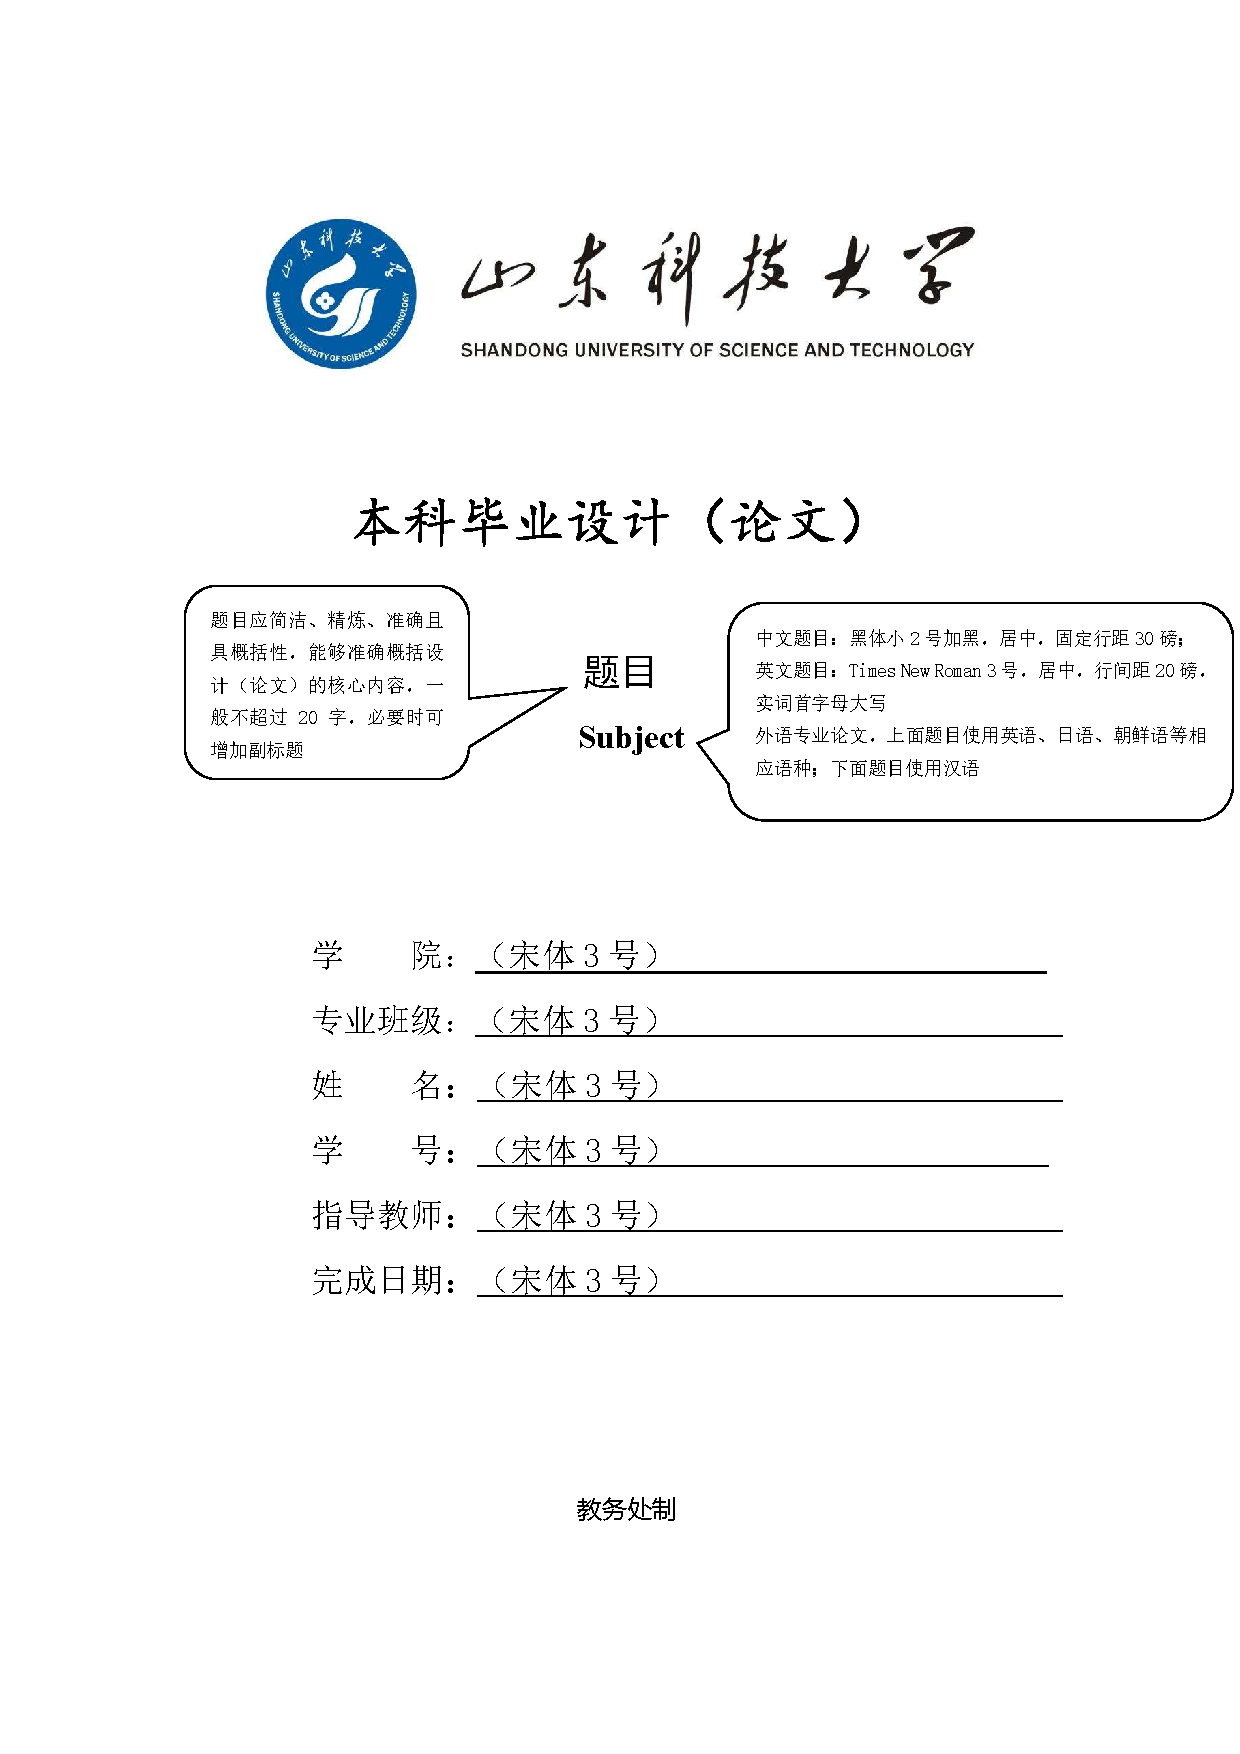
\includepdf{cover.pdf}

\tikzset{
    state/.style={circle, draw, minimum size=1cm},
    set/.style={rectangle, draw, inner sep=0.3cm, dashed}
}

% 声明
\pagenumbering{gobble}

\fancyhead[R]{\fontsize{9}{13}\selectfont \songti \textnormal{声明}} % 右侧页眉内容,不加粗

\begin{center}
  \heiti\zihao{-2}
  \setlength{\baselineskip}{1.0\baselineskip}
  \vspace*{-0.5\baselineskip}
  \textbf{学位论文原创性声明}
  \vspace*{0.5\baselineskip}
\end{center}


\KaiTi\zihao{-3}
\newlength{\zhwidth}
\settowidth{\zhwidth}{\KaiTi\zihao{-3}汉字}  % 替换“汉字”为任意两个汉字
\setlength{\parindent}{\zhwidth} % 首行缩进两个字符
\setlength{\baselineskip}{20pt}

\punctstyle{quanjiao}

% 在此处输入声明的内容
\indent 本人呈交给山东科技大学的学位论文,除所列参考文献和世所公认的文献外,全部是本人攻读学位期间在导师指导下的研究成果。除文中已经标明引用的内容外,本论文不包含任何其他个人或集体已经发表或撰写过的研究成果。对本文的研究做出贡献的个人和集体,均已在文中以明确方式标明。本人完全意识到本声明的法律结果由本人承担。\\
\indent 若有不实之处,本人愿意承担相关法律责任。
\vspace{-2ex} % 调整 tabular 之前的间距
\begin{center}
\begin{tabular}{p{8.3cm} p{6cm}}
\hspace{2.5cm} 本人签名:\raisebox{-0.5\height}{
\includegraphics[width=3cm]{my.jpg}} \rule{3cm}{0.0pt} & 日 \hspace{0.3em} 期: xxx 年 x 月 x 日 \\
\end{tabular}
\end{center}

\vspace*{2\baselineskip}

\begin{center}
  \heiti\zihao{-2}
  \setlength{\baselineskip}{1.0\baselineskip}
  \vspace*{-0.5\baselineskip}
  \textbf{学位论文使用授权声明}
  \vspace*{0.5\baselineskip}
\end{center}

\KaiTi\zihao{-3}
\settowidth{\zhwidth}{\KaiTi\zihao{-3}汉字}  % 替换“汉字”为任意两个汉字
\setlength{\parindent}{\zhwidth} % 首行缩进两个字符
\setlength{\baselineskip}{20pt}

% 在此处输入声明的内容
\indent 本人完全了解山东科技大学有关保留、使用学位论文的规定,同意本人所撰写的学位论文的使用授权按照学校的管理规定处理。\\
\indent 作为申请学位的条件之一,学校有权保留学位论文并向国家有关部门或其指定机构送交论文的电子版和纸质版;有权将学位论文的全部或部分内容编入有关数据库发表,并可以以电子、网络及其他数字媒体形式公开出版;允许学校档案馆和图书馆保留学位论文的纸质版和电子版,可以使用影印、缩印或扫描等复制手段保存和汇编学位论文;为教学和科研目的,学校档案馆和图书馆可以将公开的学位论文作为资料在档案馆、图书馆等场所或在校园网上供校内师生阅读、浏览。\\
\indent (保密的学位论文在解密后适用本授权)

\begin{center}
\begin{tabular}{p{6cm} p{1.5cm} p{6cm}}
作者签名:
\includegraphics[width=2cm]{my.jpg} & & 导师签名:

\includegraphics[width=1.5cm]{teacher.png} \\
\end{tabular}
\end{center}
\begin{center}
\begin{tabular}{p{6cm} p{1.5cm} p{6cm}}
日 \hspace{0.5cm} 期: xxx 年 x 月 x 日 & & 日 \hspace{0.5cm} 期: xxx 年 x 月 x 日 \\
\end{tabular}
\end{center}

% 中文摘要
\clearpage

\pagenumbering{Roman}
\fancyfoot[C]{\fontsize{9}{11}\selectfont\thepage}

\fancyhead[R]{\fontsize{9}{13}\selectfont \songti \textnormal{摘要}} % 右侧页眉内容,不加粗

\begin{center}
  \heiti\zihao{-2}
  \setlength{\baselineskip}{1.0\baselineskip}
  \vspace*{-0.5\baselineskip}
  \textbf{摘要}
  \vspace*{0.5\baselineskip}
\end{center}

\SimSun
\zihao{-4}
\setlength{\baselineskip}{20pt}
\setlength{\parindent}{2em} % 首行缩进两个字符
一些内容

\textbf{关键词:} 一些内容


% 英文摘要
\clearpage

\fancyhead[R]{\fontsize{9}{13}\selectfont \songti \textnormal{ABSTRACT}} % 右侧页眉内容,不加粗

\begin{center}
  \timesnewroman\zihao{-2}\bfseries
  \setlength{\baselineskip}{1.0\baselineskip}
  \vspace*{-0.5\baselineskip}
  ABSTRACT
  \vspace*{0.5\baselineskip}
\end{center}

\timesnewroman
\zihao{-4}
\setlength{\baselineskip}{20pt}

\indent some content

\textbf{Keywords: content}  % Keywords加粗


\clearpage
\fancyhf{}  % 清除之前的页眉页脚设置
\pagestyle{tocstyle}
\setstretch{2} % 设置目录的行距为1.5倍
\tableofcontents


\clearpage

\pagestyle{fancy}
\fancyhf{}  % 清除之前的页眉页脚设置
\fancyhead[L]{\fontsize{9}{13}\selectfont \songti 山东科技大学毕业设计(论文)}  % 左侧页眉设置
\fancyhead[R]{\zihao{-5} \selectfont \songti \textnormal{\leftmark}}  % 右侧页眉显示章节标题,并设置为灰色
\fancyfoot[C]{\fontsize{9}{13}\selectfont \timesnewroman \thepage}  % 页脚中间显示页码
\renewcommand{\headrulewidth}{0.4pt}  % 页眉下的分隔线宽度

% 一级标题格式
\titleformat{\chapter}[hang]{\heiti\zihao{3}\bfseries\centering}{第\,\thechapter\,章}{0.5em}{}
\titlespacing*{\chapter}{0pt}{0.5\baselineskip}{0.5\baselineskip}

% 二级标题格式
\titleformat{\section}[hang]{\heiti\zihao{4}\bfseries}{\thesection}{0.5em}{}
\titlespacing*{\section}{0pt}{0.5\baselineskip}{0.5\baselineskip}

% 三级标题格式
\titleformat{\subsection}[hang]{\heiti\zihao{-4}\bfseries}{\thesubsection}{0.5em}{}
\titlespacing*{\subsection}{0pt}{0.5\baselineskip}{0.5\baselineskip}

% 正文格式
\renewcommand{\thepage}{\arabic{page}}  % 切换为阿拉伯数字页码
\setcounter{page}{1}  % 重置页码计数
\SimSun
\zihao{-4}
\setlength{\baselineskip}{20pt}
\setlength{\parindent}{2em} % 首行缩进两个字符
\setlength{\parskip}{0pt}  % 段前段后间距均为0行
\renewcommand{\baselinestretch}{1}  % 单倍行距

\chapter{第1章\ 一些内容}\label{ux7b2c1ux7ae0-ux7eeaux8bba}

\section{1.1 一些内容}\label{11-ux7814ux7a76ux80ccux666f}

\subsection{1.1.1
一些内容}\label{111-ux5206ux5e03ux5f0fux8ba1ux7b97ux6846ux67b6ux7684ux6f14ux53d8}

一些内容



\section{1.2 一些内容}\label{12-ux7814ux7a76ux610fux4e49}

一些内容


\chapter{第2章\
一些内容}\label{ux7b2c2ux7ae0-ux4e00ux79cdux6700ux5c0fux5316ux901aux4fe1ux91cfux7684ux4e9aux7ebfux6027ux52a8ux6001ux56feux5206ux5272ux7b97ux6cd5}
\section{2.1 一些内容}
行内公式样例:\\
设 \( M \) 是 Map 函数,\( R \) 是 Reduce 函数。对于输入数据集 \( D = \{d_1, d_2, \ldots, d_n\} \),Map 函数处理数据项 \( d_i \),生成一组中间键值对 \( (k, v_i) \):
\[
M(d_i) = \{(k, v_1), (k, v_2), \ldots, (k, v_m)\}。 \tag{2.1}
\]

然后,相同键 \( k \) 的所有值集合 \( V_k = \{v_1, v_2, \ldots, v_m\} \) 被送到同一个 Reduce 任务,由 Reduce 函数处理:

\[
R(k, V_k) = \text{some function of } V_k, \tag{2.2}
\]

\noindent Reduce 函数的输出是对每个键 \( k \) 的聚合结果。

\begin{figure}
\centering

\begin{tikzpicture}[
    auto,
    block/.style={rectangle, draw, fill=blue!20, text width=4em, text centered, rounded corners, minimum height=2.5em, font=\small},
    line/.style={draw, -Latex},
    bigblock/.style={draw, thick, fill=blue!10, text width=5em, align=center, minimum height=10em, font=\small}
]

% Nodes
\node[block] (input) {Input Data};
\node[bigblock, right=of input, yshift=-1cm] (map) {Map Functions};
\node[block, right=of map] (shuffle) {Shuffle and Sort};
\node[bigblock, right=of shuffle, yshift=-1cm] (reduce) {Reduce Functions};
\node[block, right=of reduce] (output) {Output Data};

% Positions for mappers and reducers
\foreach \i in {1,2,3}
{
    \node[block, below of=map, node distance=1.5*\i cm] (mapper\i) {Mapper \i};
    \node[block, below of=reduce, node distance=1.5*\i cm] (reducer\i) {Reducer \i};
}

% Draw arrows
\draw[line] (input) -- (map);
\draw[line] (map) -- (shuffle);
\draw[line] (shuffle) -- (reduce);
\draw[line] (reduce) -- (output);

% Connect mappers and reducers
\foreach \i in {1,2,3}
{
    \draw[line] (mapper\i) -- (shuffle);
    \draw[line] (shuffle) -- (reducer\i);
}

\end{tikzpicture}
\caption{\songti\bfseries\zihao{5} 图 2.1 tikz样例}
\end{figure}

\section{2.2 一些内容}
\subsection{2.2.1 一些内容}
一些内容

\subsubsection{Actor模型的核心概念}\label{actorux6a21ux578bux7684ux6838ux5fc3ux6982ux5ff5}

一些内容

\begin{figure}[ht]
    \centering
    \vspace{1em} % 在图形上方添加一个空行
    \begin{tikzpicture}[
        actor/.style={rectangle split, rectangle split parts=2, draw, minimum width=2.5cm, minimum height=1.5cm, font=\sffamily\bfseries, rectangle split part align=center},
        mailbox/.style={rectangle, draw, dashed, minimum width=2.5cm, minimum height=1cm, font=\sffamily\footnotesize, align=center},
        message/.style={-Stealth, thick, draw},
        process/.style={message, dashed},
        node distance=4cm and 5cm
    ]

    % Actors
    \node[actor] (A1) {Actor 1\nodepart{second}Internal State};
    \node[actor, right=of A1] (A2) {Actor 2\nodepart{second}Internal State};
    \node[actor, below=of A1] (A3) {Actor 3\nodepart{second}Internal State};
    \node[actor, right=of A3] (A4) {Actor 4\nodepart{second}Internal State};

    % Mailboxes
    \node[mailbox, below=1cm of A1] (M1) {Mailbox};
    \node[mailbox, below=1cm of A2] (M2) {Mailbox};
    \node[mailbox, below=1cm of A3] (M3) {Mailbox};
    \node[mailbox, below=1cm of A4] (M4) {Mailbox};

    % Messages
    \draw[message] (A1) -- (M2) node[midway, above] {Msg 1};
    \draw[message] (A2) -- ++(2,0) -- ++(0,-7) -- (M4) node[midway, above ,yshift=95pt ,xshift=-10pt] {Msg 2}; % Adjusted position
    \draw[message] (A4) -- (M3) node[midway, below] {Msg 3};
    \draw[message] (A3) -- (M1) node[midway, left] {Msg 4};
    \draw[message] (A1) -- (M4) node[midway, sloped, above] {Msg 5};

    % Processing arrows
    \draw[process] (M1) -- (A1) node[midway, left] {Process};
    \draw[process] (M2) -- (A2) node[midway, left] {Process};
    \draw[process] (M3) -- (A3) node[midway, left] {Process};
    \draw[process] (M4) -- (A4) node[midway, left] {Process};

    \end{tikzpicture}
    \caption{\songti\bfseries\zihao{5} 图3.4 复杂tikz样例}
\end{figure}
\subsubsection{一些内容}\label{ux5b9eux9645ux5e94ux7528}

一些内容

\subsection{3.4.2 一些内容}\label{242-ux6570ux5b66ux8868ux793a}

\textbf{定义 3.2 Caputo分数阶导数 Podlubny,1999\upcite{podlubny1999fractional}:}

复杂公式样例:
\\
\[
\begin{cases}
\vphantom{\displaystyle \sum_{i=1}^n} B_u^{v_i}(t) = \max\left(B_u^{v_i}(t^{v_i}) + \left(-\lambda \ln(1 + \gamma B_{u}^{avg}) \cdot (t - t^{v_i}) \right), 0\right), \\[13pt]
\displaystyle \partial^{\mathrm{mac(v_i)}} {}^{C} \mathcal{D}^\alpha B_u(t) = \sum_{\mathrm{mac(v_i)}} (B_{m(v_i)}(t^{v_i})+1) \cdot F(E(u,m(v_i))) \\
\phantom{\displaystyle \partial^{\mathrm{mac(v_i)}} {}^{C} \mathcal{D}^\alpha B_u(t) = } + G(u) - G(v_i)。
\end{cases} \tag{3.18}
\] 

\section{3.6 一些内容}\label{26-ux5b9eux9a8cux4e0eux4effux771f}

一些内容
\subsection{3.6.1 一些内容}\label{261-ux7ea2ux9ed1ux6811ux4efbux52a1}
一些内容
\\
\begin{figure}[H]
    \centering
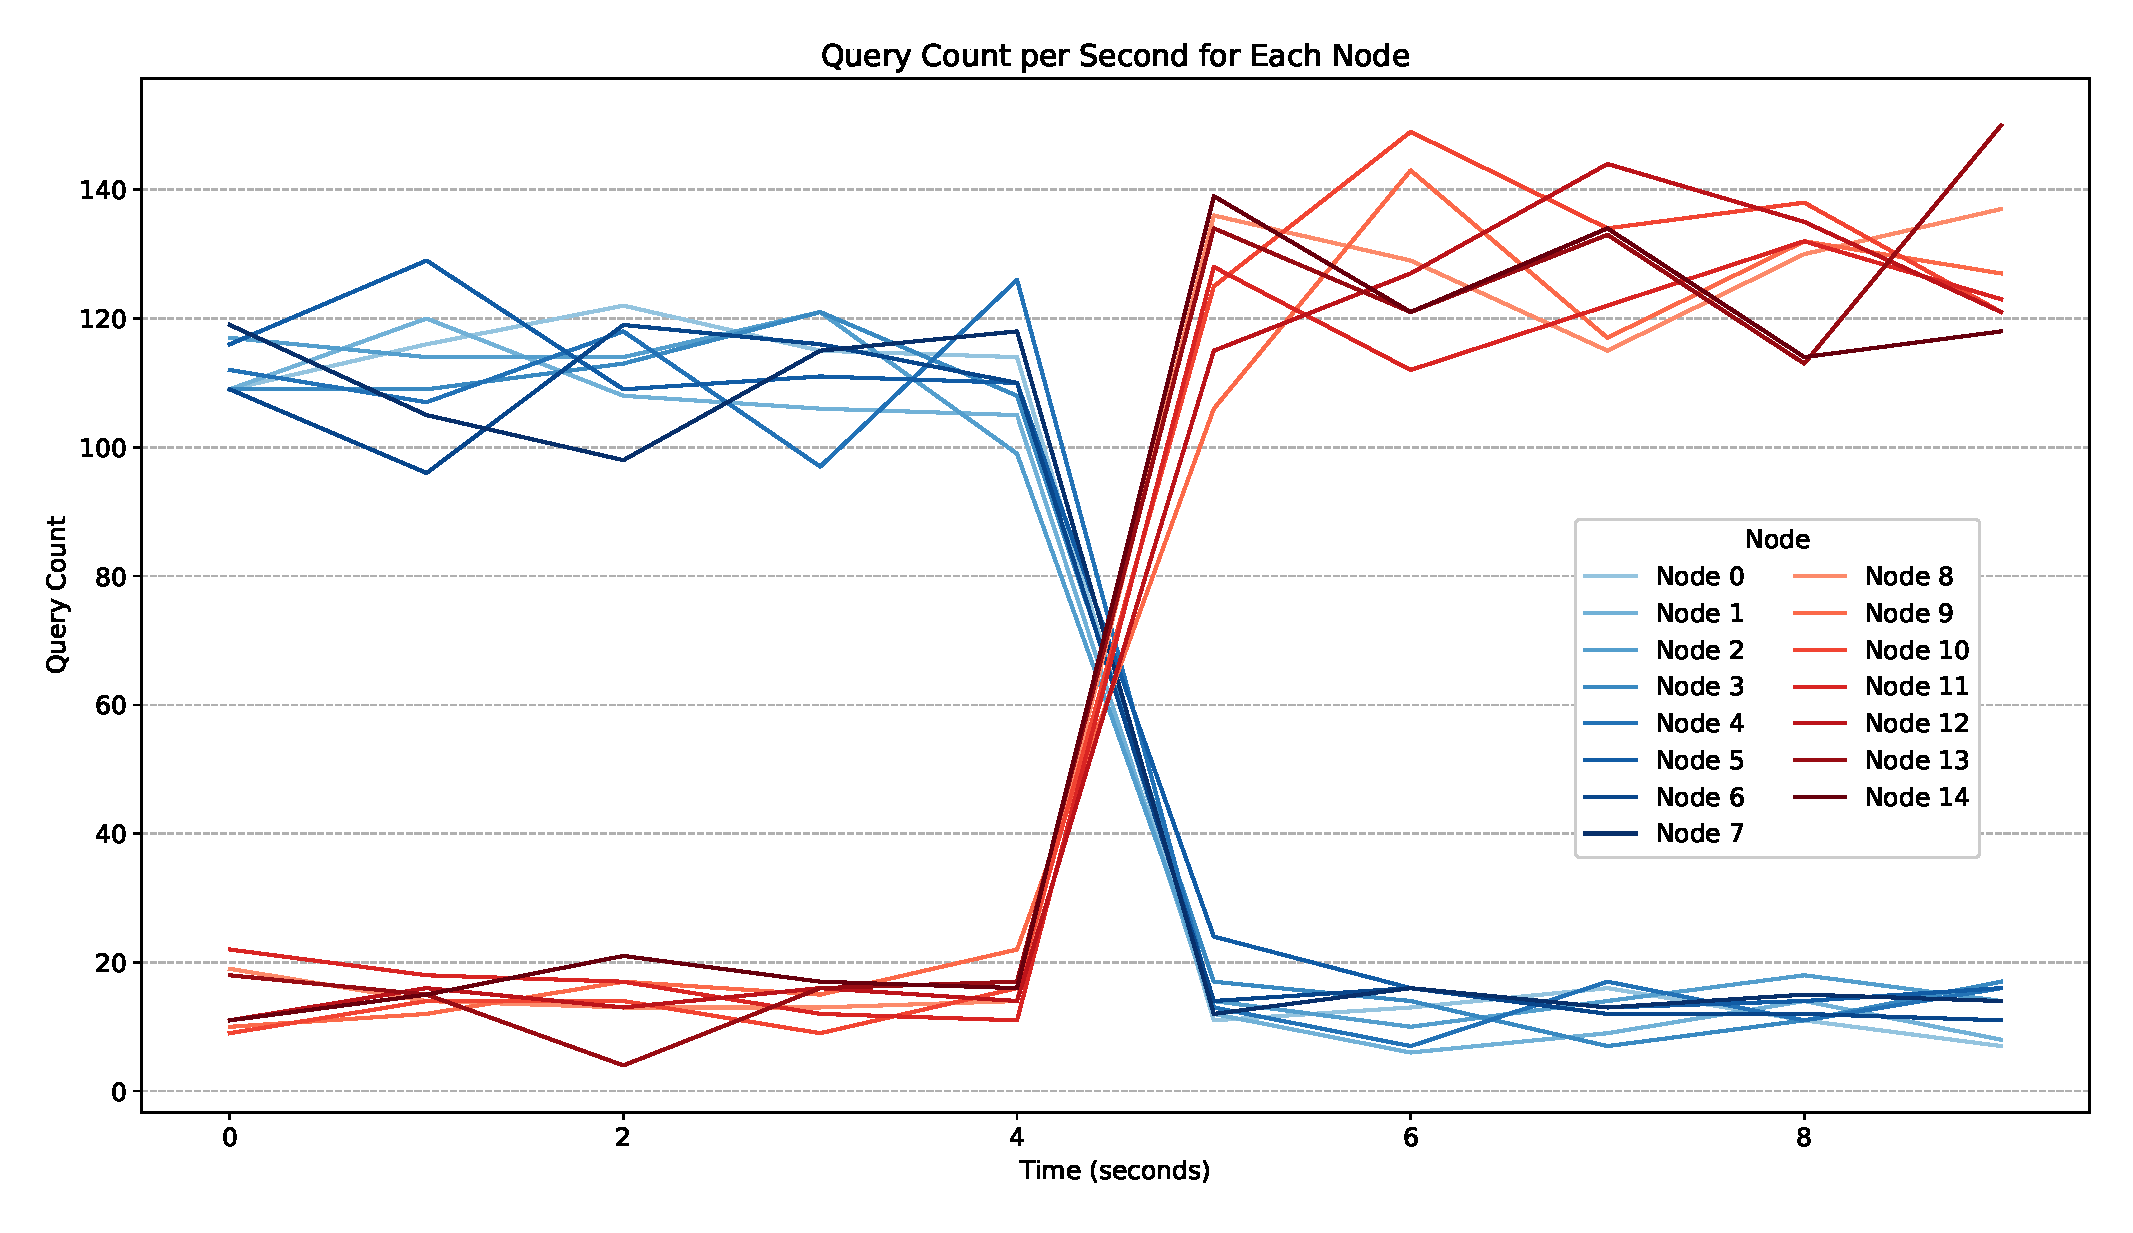
\includegraphics{node_query_count_over_time.eps}
    \caption{\songti\bfseries\zihao{5} 图 3.6 外部矢量图样例}
\end{figure}
\noindent \textbf{一些内容:} 

\begin{table}[h]
    \centering
    \captionsetup{labelformat=empty, position=bottom}
    \caption{\songti\bfseries\zihao{5} 表 3-1 一些内容}
    \begin{tabular}{cccc}
        \toprule
        id & A & B & C \\
        \midrule
        1 & 0 & 0.0 & create root \\
        2 & (x,x) & 0.0 & xxx \\
        3 & (x,x) & 0.0 & xxx \\
        4 & (x,x) & 0.0 & xxx \\
        5 & (x,x) & 0.0 & xxx \\
        ... & ... & ... & ... \\
        15 & x & 0.0 & query \\
        16 & x & 0.xxxxxxxxxxxxxxxxxx & yyy \\
        17 & x & 0.xxxxxxxxxxxxxxxxxx & yyy \\
        18 & x & 0.xxxxxxxxxxxxxxxxxx & yyy \\
        19 & x & 0.xxxxxxxxxxxxxxxxxx & yyy \\
        \bottomrule
    \end{tabular}
\end{table}

引用样例:
参考文献\cite{li2012finite} 和 开源仓库\cite{aburn2019fodeint}。被文献\cite{LIU2024106124}等广泛的使用。

\chapter{第4章\ 
一些内容}\label{ux7b2c3ux7ae0-gorest-ux4e00ux79cdux57faux4e8eux56feux7684ux7075ux6d3bux7684ux5927ux6570ux636eux8ba1ux7b97ux6846ux67b6ux6a21ux578b}

\section{4.1 一些内容}\label{31-ux56feux4e0eux8ba1ux7b97}

\subsection{4.1.1
一些内容}\label{343-gorestux4efbux52a1ux6d41ux7a0b}

一些内容
\begin{figure}[H]
\begin{center}
\scalebox{0.7}{
\begin{tikzpicture}[node distance=2cm and 2cm, auto]
% Nodes
\node (A) [process] {A};
\node (B) [decision, below of=A, yshift=-1cm] {B};
\node (C) [process, below right=of B, xshift=1cm] {C};
\node (D) [process, below left=of B, xshift=-1cm] {E};
\node (F) [process, below of=B, yshift=-1cm] {G};

% Paths
\draw [arrow] (A) -- (B);
\draw [arrow] (B) -| node[anchor=north, near start] {yes} (C);
\draw [arrow] (B) -| node[anchor=north, near start] {no} (D);
\draw [arrow] (D) -- (F);

\end{tikzpicture}
}

\caption{\songti\bfseries\zihao{5} 图 4.2 一些内容}
\end{center}
\end{figure}

\subsection{4.5 一些内容}
一些内容

\begin{figure}
\centering
\begin{tikzpicture}
\begin{axis}[
    title={some content},
    xlabel={Data Range ($\times 10^7$)},
    ylabel={Time (seconds)},
    grid=major,
    legend style={at={(0.95,0.3)},anchor=north east}, % 图例位置在右上角内部
    width=0.9\textwidth, % 调整宽度
    height=0.45\textwidth,  % 调整高度以保持长方形形状
    scaled x ticks=false, % 不自动缩放x轴刻度
    tick label style={/pgf/number format/fixed}, % 使用固定点数表示
    xtick={1000000,2000000,...,10000000}, % 自定义刻度
    xticklabels={1,2,3,4,5,6,7,8,9,10} % 自定义刻度标签
]
\addplot[
    color=blue,
    mark=o,
    thick
] coordinates {
    (2000000, 0.361797789)
    (3000000, 0.228487892)
    (4000000, 0.236640184)
    (5000000, 0.2447254)
    (6000000, 0.267326046)
    (7000000, 0.239472694)
    (8000000, 0.29180491)
    (9000000, 0.265192163)
    (10000000, 0.331729165)
};
\legend{xxx}

\addplot[
    color=red,
    mark=x,
    thick
] coordinates {
    (1000000, 0.060728656)
    (2000000, 0.103753581)
    (3000000, 0.147702729)
    (4000000, 0.234056287)
    (5000000, 0.266536737)
    (6000000, 0.323095286)
    (7000000, 0.386735194)
    (8000000, 0.395468254)
    (9000000, 0.458787718)
    (10000000, 0.513965945)
};
\legend{xxx, yyy}
\end{axis}
\end{tikzpicture}
\caption{\songti\bfseries\zihao{5} 图 xxx 一些内容}
\end{figure}



\chapter{第5章\ 
一些内容}\label{ux7b2cux56dbux7ae0ux603bux7ed3ux4e0eux5c55ux671b}

\section{5.1
一些内容}\label{41-ux4e3bux8981ux7814ux7a76ux6210ux679cux603bux7ed3}
\subsection{5.1.1
一些内容}
一些内容
\textbf{(1)一些内容:}
一些内容
\subsection{5.1.2
一些内容}
一些内容
\textbf{(1)一些内容:}
一些内容
\section{5.2
一些内容}\label{43-ux9762ux4e34ux7684ux6311ux6218ux4e0eux6539ux8fdbux65b9ux5411}
\subsection{5.2.1
一些内容}
一些内容
\textbf{(1)一些内容:}

一些内容

\subsection{5.2.2
一些内容}
一些内容
\textbf{(1)一些内容:}

一些内容

% 参考文献
\clearpage % 结束时清除页面

\addcontentsline{toc}{chapter}{参考文献}

\fancyhead[R]{\fontsize{9}{13}\selectfont \songti \textnormal{参考文献}} 

\chapter*{\fontsize{18pt}{22pt}\selectfont 参考文献}

\printbibliography

\clearpage % 结束时清除页面

\chapter*{\fontsize{18pt}{22pt}\selectfont 致谢}
\addcontentsline{toc}{chapter}{致谢}
\markboth{致谢}{致谢}
\begin{acknowledgements}
一些内容
\end{acknowledgements}


\end{document}
